\documentclass[11pt, a4paper]{article}

\usepackage[english,francais]{babel}
\usepackage[utf8]{inputenc}
\usepackage[T1]{fontenc}
\usepackage[pdftex]{graphicx}
\usepackage{setspace}
\usepackage[french]{varioref}
\usepackage{amsfonts}
\usepackage{amssymb}
\usepackage{geometry}
\usepackage{amsthm}
\usepackage{enumerate}
\usepackage[french, ruled]{algorithm2e}
\geometry{margin=2cm}

\usepackage{tikz}
\usetikzlibrary{calc}   % coordinate calculation
\usepackage{xifthen}

\title{Correctness}
\author{\'Eloi Perdereau}
%\date{}

\newcommand{\spacee}[2] {
  \begin{tikzpicture}[thick, scale=0.6]
    \def \step {1}
    \def \cc {\step/2}  % center of cell
    \coordinate (offset) at ($(\cc,\cc)$);
    \draw[step=\step] (0,0) grid ($#1$);   % draw the grid, base at #1
    % draw the neighbors
    \foreach \coord in #2 {
      \coordinate[at=\coord, name=A];
      \draw ($(A) + (offset)$) circle ({\cc*0.8});
    }
  \end{tikzpicture}
}

\theoremstyle{plain}
\newtheorem{thm}{Theorem}[section]
\newtheorem{lem}[thm]{Lemma}
\newtheorem{prop}[thm]{Proposition}
\newtheorem*{cor}{Corollary}

\theoremstyle{definition}
\newtheorem{defn}{Definition}[section]
\newtheorem{conj}{Conjecture}[section]
\newtheorem{exmp}{Example}[section]

\theoremstyle{remark}
\newtheorem*{rem}{Remark}
\newtheorem*{note}{Note}

\begin{document}

\maketitle

We define the \textit{bounding box} $BB(t)$ of the robots as the smallest
enclosing rectangle (oriented with the grid's axes) which contains all robots
at step $t$.

\begin{prop}
When following the algorithm described above, the bounding box of the robots is
monotonically non-inflating, i.e., $BB(t+1) \subseteq BB(t)$ for all $t$.
\end{prop}

\section{A single robot on the topmost row}

We note $r(t)$ the single robot in the topmost row of the bounding box at step
$t$. If there are more than one robot, $r(t)$ is not defined.

\begin{prop}
If $r(t)$ exists and is on $(0,i)$, then there was a robot on $(0,i-1)$, $(0,i)$
or $(0,i+1)$ at step $t-1$.
\end{prop}

This shows that studying the neighborhood of $r(t)$ for new robots on the
topmost row is enough for the whole row.

\begin{lem}
If $r(t)$ exists and there are at least three robots in the space, then after a
constant number of steps, either $BB(t+c) \subset BB(t)$ (the topmost row moves
down) or it becomes an end case
\end{lem}

\begin{proof}

We define the graph $G_{single}(V_{single}, E_{single})$ as follows :
\begin{itemize}
  \item $V_{single}$ : neighborhood cases of $r(t)$
  \item $(u,v) \in E_{single}$ if $u$ can lead to $v$ at $t+1$ for any robot on
        row $i$, and $t+1$ is not an end case.
\end{itemize}
The graph have been generated and is shown on figure \ref{graph:single}. We
notice multiple cycles, i.e. row $0$ might never move down. However, edges are
only representative for one step. In other words, there are paths that $r(t)$
cannot go through. We will study 4 of them and it will be enough to prove that
$BB(t+c) \subset BB(t)$. \\

\noindent
Note $A$ to $G$ the 7 nodes of $G_{single}$ from top to bottom and left to
right. \\
Left moves are when $r(t) > r(t+1)$, mid moves and right moves are defined
analogously. \\
The middle robot in the start node is at $(0,0)$ at $t$.
\begin{itemize}
  \item path($D \rightarrow A \rightarrow B$) : $D \rightarrow A$ and $A
  \rightarrow B$ are respectively a left and a right move.
  \begin{enumerate}[a.]
    \item In order to have $(0,-1)$ filled at $t+1$, $(0,1)$ must be on case
          $1.2.6$ ($-90^{\circ}$) at $t$. So $(1,-1)$, $(1,0)$ and $(1,1)$ are
          empty at $t$.
    \item Giving a., in order to have $(1,-1)$ empty at $t+1$, $(1,-1)$ must be
          on case $1.3.5$ at $t$. So at $t+1$, $(2,-1)$ will be filled.
    \item[c1.] In order to have $(0,0)$ filled at $t+2$, $(0,1)$ must be on case
          $1.2.5$ or $1.3.6$ (both $+180^{\circ}$). Which is impossible because
          of b.
    \item[c2.] Giving b., there is no way $(0,0)$ can be filled at $t+2$.
  \end{enumerate}
  Therefore if $r(t)$ pass through $D \rightarrow A$, $r(t+1)$ cannot pass
  through $A \rightarrow B$. This invalidates all cycles involving both $D$ and
  $A$.
\end{itemize}

\end{proof}

\begin{figure}
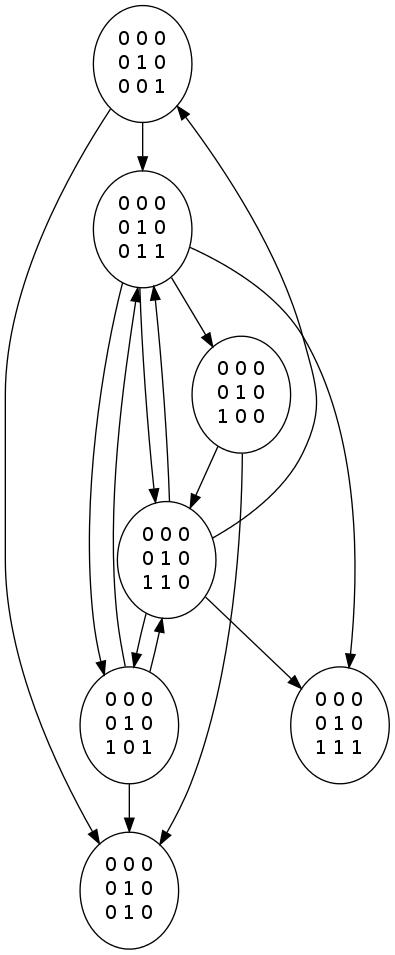
\includegraphics[scale=0.50]{graph_single_all.jpg}
\caption{Single robot}
\label{graph:single}
\end{figure}

\begin{figure}
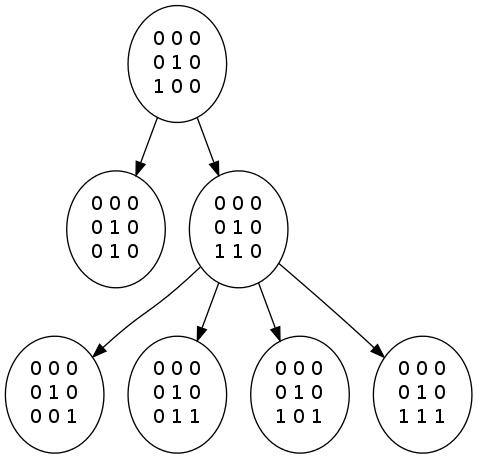
\includegraphics[scale=0.50]{graph_single_left.jpg}
\caption{Single robot : left moves}
\label{graph:single_left}
\end{figure}

\begin{figure}
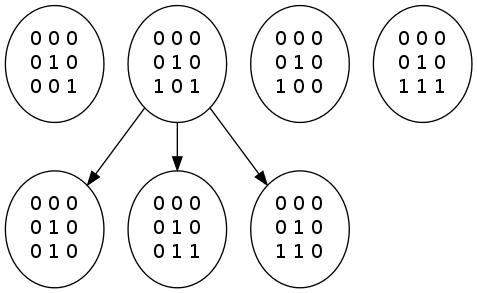
\includegraphics[scale=0.50]{graph_single_mid.jpg}
\caption{Single robot : mid moves}
\label{graph:mid}
\end{figure}

\begin{figure}
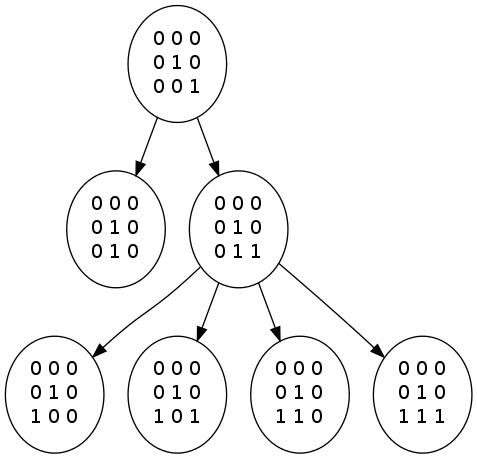
\includegraphics[scale=0.50]{graph_single_right.jpg}
\caption{Single robot : right moves}
\label{graph:right}
\end{figure}

\section{More than one robot on the topmost row}

\begin{figure}
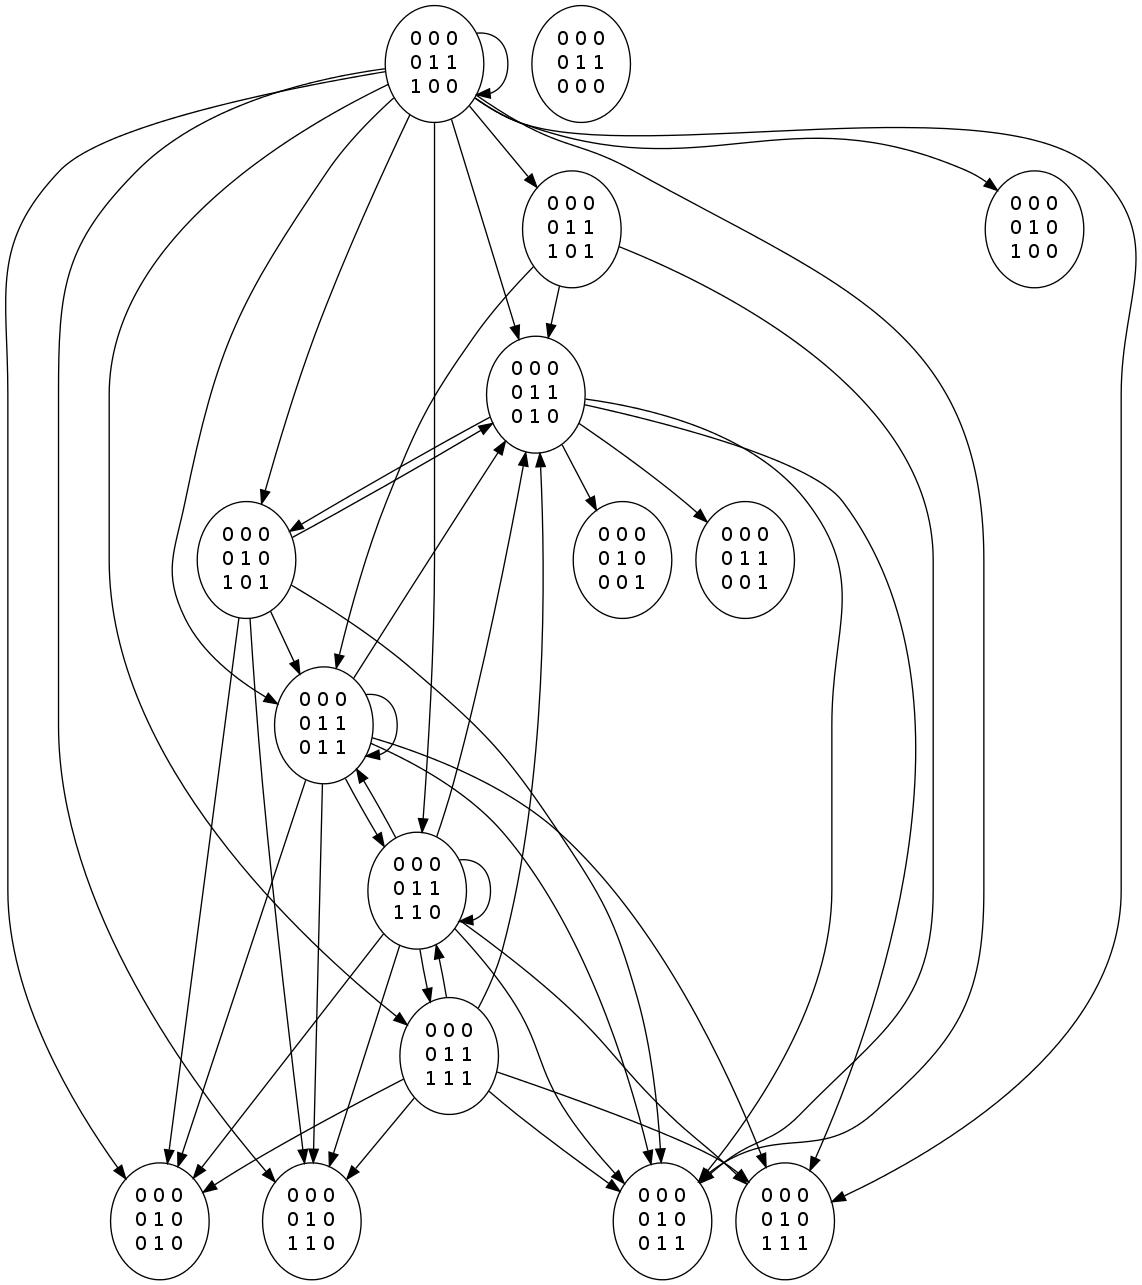
\includegraphics[scale=0.50]{graph_leftmost_mid.jpg}
\caption{Mid moves}
\label{graph:leftmost_mid}
\end{figure}

\begin{figure}
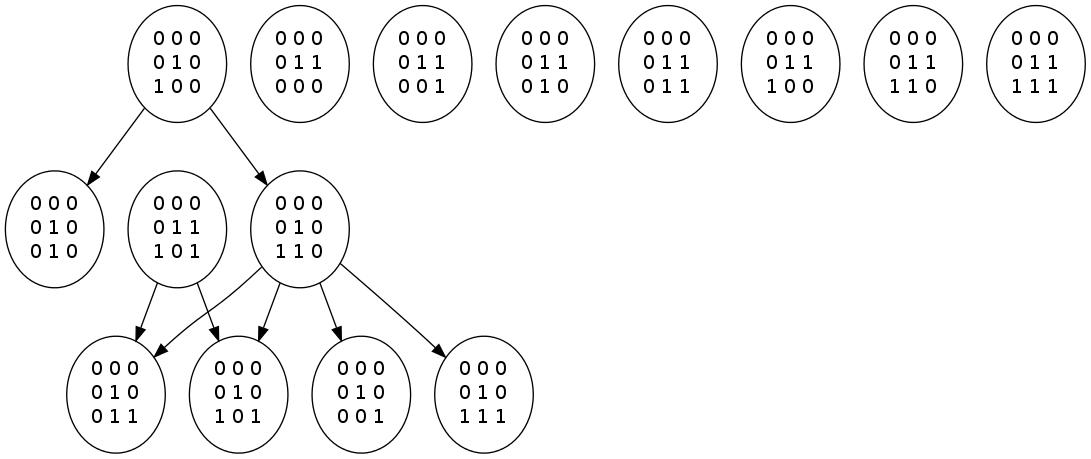
\includegraphics[scale=0.50, angle=00]{graph_leftmost_left.jpg}
\caption{Left moves}
\label{graph:leftmost_left}
\end{figure}

\end{document}
